\documentclass[../main.tex]{subfiles}
\begin{document}
\section{Results}
\subsection{$2 \times 2$ lattice, analytical expressions}
If we scale the value of $\beta$ from $1/k_BT$ to $1/J$ (Scaling factor $k_B T/J$) in the analytical expression from section \ref{sec:theory-analy}, we will get a good benchmark for computer computations to come. These values are listed in table \ref{tab:2x2spinsEnergiesMags} below. Note that all values are divided by four, since we want the values per bond, and not for the entire lattice.
\begin{table}[!h]
\begin{center}
  \begin{tabular}{| l | r |}
    \hline
    \textbf{Mean energy,} $\mathbf{\langle E \rangle}$ & $-1.9960$  \\
    \hline
    \textbf{Mean absolute magnetization,} $\mathbf{\langle |\mathcal{M}| \rangle}$ & $0.9987$ \\
    \hline
    \textbf{Specific heat capacity,} $\mathbf{C_V}$ & $0.0321$\\
    \hline
    \textbf{Susceptibility,} $\mathbf \chi$ & $3.9933$ \\
    \hline
  \end{tabular}
  \caption{Benchmark for material characteristics per bond for a $2 \times 2$ lattice}
  \label{tab:2x2spinsEnergiesMags}
\end{center}
\end{table}
\FloatBarrier

\subsection{Ising model: simulation over temperature}
We ran the program for different amounts of Monte Carlo cycles and plottet the error (analytical - simulated) in figure \ref{fig:results-MCplot} below. It seems we want to use around $10^{7}$ MC cycles or more to get a good simulation.

\begin{figure}[!h]
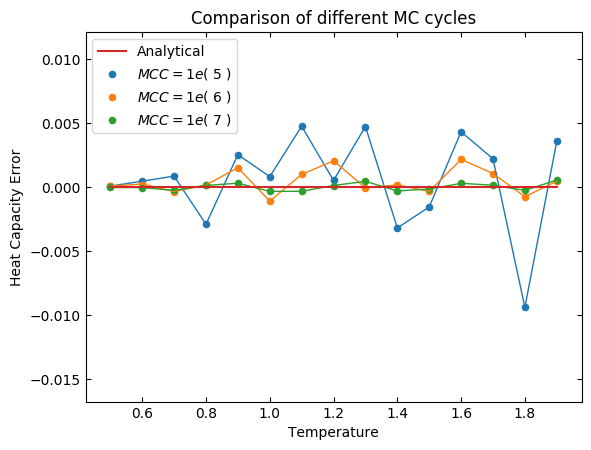
\includegraphics[scale=0.7]{CyclesComparison.png}
\caption{Shows the accuracy of different amount of MC cycles over temperature.}
\label{fig:results-MCplot}
\end{figure}
\FloatBarrier

\subsection{$20 \times 20$ lattice, analytical expressoins}
% T = 1.0(kT/J):
% Mean energy and magnetization func of MC cycles:
% Ordnet orientering: Program initilize.cpp (For T < 1.5 så er alle spinn opp,
% ellers spinn ned)

% sett inn følgende bilder fra mappe M+E under img:
% T1_1.png
% T1_2.png
% Tekst: ordnet spinn orientering for T= 1.0

% Random spinn orientering: Program initilize_random (Setter spinn ned(-1)
% hvis verdien vi får mellom 0 og 1 er mindre eller lik 0.5 ).

% sett inn følgende bilder fra mappe M+E under img:
% L20T1random_1.png
% L20T1random_2.png
% Tekst: Random spinn orientering for T = 1.0


% Likevekt:

% T = 2.4(kT/J):
% Mean energy and magnetization func of MC cycles:
% Ordnet orientering: Program initilize.cpp (For T < 1.5 så er alle spinn opp,
% ellers spinn ned)

% sett inn følgende bilder fra mappe M+E(ligger inni img):
% T2_1.png
% T2_2.png
% Tekst: ordnet spinn orientering for T= 2.4

% Random spinn orientering: Program initilize_random (Setter spinn ned(-1)
% hvis verdien vi får mellom 0 og 1 er mindre eller lik 0.5 ).

% L20T1random_1.png
% L20T1random_2.png
% Tekst: Random spinn orientering for T = 2.4


% Likevekt:

% Oversiktelig tabell med når likevekt nås ca. (antall mcs)

%     Ordnet magnetisering  Random magnetisering  Ordnet energi Random energi
% T1:
% T2:

% Estimat av equilibration time:

% Antall aksepterte spinn per montecarlocycle

% Diskusjon/resultater
% Aksepterte spinn som funksjon av T:
% Økt temperatur gir flere aksepterte flips.
% Setter man startpoint til random går den fortere mot likevekt ?


\end{document}
